\documentclass[10pt, landscape]{article}
\usepackage[scaled=0.92]{helvet}
\usepackage{calc}
\usepackage{multicol}
\usepackage{ifthen}
\usepackage[a4paper,margin=3mm,landscape]{geometry}
\usepackage{amsmath,amsthm,amsfonts,amssymb}
\usepackage{color,graphicx,overpic}
\usepackage{hyperref}
\usepackage{newtxtext} 
\usepackage{enumitem}
\usepackage[table]{xcolor}
\usepackage{mathtools}
% for drawing diragrams/graphs
\usepackage{tikz}
\usetikzlibrary{arrows.meta}
\usetikzlibrary{calc}
\graphicspath{ {./images/} }
\setlist{nosep}

% ADDITIONAL USEFUL PACKAGES:
% for matrices
\usepackage{nicematrix}
% for relations
\usepackage{cancel}
\usepackage{ mathrsfs }
% for including images
\graphicspath{ {./images/} }


\pdfinfo{
  /Title (MA1102R.pdf)
  /Creator (TeX)
  /Producer (pdfTeX 1.40.0)
  /Author (Jovyn)
  /Subject (MA1102R)
  /Keywords (MA1102R, calculus,nus,cheatsheet,pdf)}

% Turn off header and footer
\pagestyle{empty}

\newenvironment{tightcenter}{%
  \setlength\topsep{0pt}
  \setlength\parskip{0pt}
  \begin{center}
}{%
  \end{center}
}

% redefine section commands to use less space
\makeatletter
\renewcommand{\section}{\@startsection{section}{1}{0mm}%
                                {-1ex plus -.5ex minus -.2ex}%
                                {0.5ex plus .2ex}%x
                                {\normalfont\large\bfseries}}
\renewcommand{\subsection}{\@startsection{subsection}{2}{0mm}%
                                {-1explus -.5ex minus -.2ex}%
                                {0.5ex plus .2ex}%
                                {\normalfont\normalsize\bfseries}}
\renewcommand{\subsubsection}{\@startsection{subsubsection}{3}{0mm}%
                                {-1ex plus -.5ex minus -.2ex}%
                                {1ex plus .2ex}%
                                {\normalfont\small\bfseries}}%
\renewcommand{\familydefault}{\sfdefault}
\renewcommand\rmdefault{\sfdefault}
%  makes nested numbering (e.g. 1.1.1, 1.1.2, etc)
\renewcommand{\labelenumii}{\theenumii}
\renewcommand{\theenumii}{\theenumi.\arabic{enumii}.}
\renewcommand\labelitemii{•}
%  convenient absolute value symbol
\newcommand{\abs}[1]{\vert #1 \vert}
%  convenient floor and ceiling
\newcommand{\floor}[1]{\lfloor #1 \rfloor}
\newcommand{\ceil}[1]{\lceil #1 \rceil}
%  convenient modulo
\newcommand{\Mod}[1]{\ \mathrm{mod}\ #1}
%  for logical not operator, iff symbol, convenient "if/then"
\renewcommand{\lnot}{\mathord{\sim}}
\let\iff\leftrightarrow
\let\Iff\Leftrightarrow
\let\then\rightarrow
\let\Then\Rightarrow
%  vectors
\newcommand{\vv}[1]{\boldsymbol{#1}}
\newcommand{\VV}[1]{\overrightarrow{#1}}
%  column vector
\newcommand{\cvv}[1]{\left(\begin{smallmatrix}#1\end{smallmatrix}\right)}

\makeatother
\definecolor{myblue}{cmyk}{1,.72,0,.38}
\everymath\expandafter{\the\everymath \color{myblue}}
% Define BibTeX command
\def\BibTeX{{\rm B\kern-.05em{\sc i\kern-.025em b}\kern-.08em
    T\kern-.1667em\lower.7ex\hbox{E}\kern-.125emX}}

% Don't print section numbers
\setcounter{secnumdepth}{0}

\setlength{\parindent}{0pt}
\setlength{\parskip}{0pt plus 0.5ex}
%% this changes all items (enumerate and itemize)
\setlength{\leftmargini}{0.5cm}
\setlength{\leftmarginii}{0.5cm}
\setlist[itemize,1]{leftmargin=2mm,labelindent=1mm,labelsep=1mm}
\setlist[itemize,2]{leftmargin=4mm,labelindent=1mm,labelsep=1mm}

%My Environments
\newtheorem{example}[section]{Example}
% -----------------------------------------------------------------------

\begin{document}
\raggedright
\footnotesize
\begin{multicols*}{4
    '}


% multicol parameters
% These lengths are set only within the two main columns
\setlength{\columnseprule}{0.25pt}
\setlength{\premulticols}{1pt}
\setlength{\postmulticols}{1pt}
\setlength{\multicolsep}{1pt}
\setlength{\columnsep}{2pt}

\begin{center}
    \fbox{%
        \parbox{0.8\linewidth}{\centering \textcolor{black}{
            {\Large\textbf{MA1102R}}
            \\ \normalsize{AY20/21 sem 2}}
            \\ {\footnotesize \textcolor{myblue}{by jovyntls}}
        }%
    }
\end{center}

\section{00. FUNCTIONS \& SETS}
\subsection{sets}
\centerline{$A = \{ x \mid \ properties \ of x \}$}
\begin{itemize}
    \item $A \subseteq B$: A is a subset of B
    \item $A \nsubseteq B$: A is not a subset of B
    \item $A = B \iff A \subseteq B \land B \subseteq A$
\end{itemize}

\subsubsection{operations on sets}
\begin{itemize}
    \item union: $A \cup B = \{x \mid x \in A \lor x \in B\}$
    \item intersection: $A \cap B = \{x \mid x \in A \land x \in B\}$
    \item difference: $A \backslash B = \{x \mid x \in A \land x \notin B\}$
\end{itemize}

\begin{center}
\setlength{\columnseprule}{0pt}
\begin{multicols*}{2}

    \subsubsection{notations of sets}
    \begin{itemize}
        \item $\mathbb{R, Q, Z, N}$
        \item $\mathbb{N} = \mathbb{Z}^+$
        \item $\emptyset$: empty set
    \end{itemize}

    \subsubsection{notations of intervals}
    \begin{itemize}
        \item closed interval (inclusive): $[a, b] = \{x \mid a \leq x \leq b\}$
        \item open interval (exclusive): $(a, b) = \{x \mid a < x < b\}$
        \begin{itemize}
            \item $(a, \infty) = \{x \mid a < x\}$
        \end{itemize}
    \end{itemize}

\end{multicols*}
\end{center}

\subsection{functions}
\begin{itemize}
    \item \textbf{existence}: $\forall a \in A, f(a) \in B$
    \item \textbf{uniqueness}: $\forall a \in A$ has only one image in $B$.
    \item for $f : A \to B$
    \begin{itemize}
        \item domain: $A$
        \item codomain: $B$
        \item range: $\{f(x) \mid x \in A\}$
    \end{itemize}
    \item for this mod: 
    \begin{itemize}
        \item $A, B \subseteq \mathbb{R}$
        \item if $A$ is not stated, the domain of $f$ is the largest possible set for which $f$ is defined
        \item if $B$ is not stated, $B = \mathbb{R}$
    \end{itemize}
\end{itemize}

\subsubsection{graphs of functions}
\begin{tightcenter}
    The graph of $f$ is the set 
    \\ $G(f) := \{ \left(x, f(x)\right) \mid x \in A\}$
\end{tightcenter}
\begin{itemize}
    \item if $A, B \subseteq R$ then $G(f) \subseteq A \times B \subseteq \mathbb{R} \times \mathbb{R}$
    \item each element is a point on the Cartesian plane $\mathbb{R}^2$
\end{itemize}

\subsubsection{algebra of functions}
% \begin{center}
%     addition
%     \\* $(f+g)(x) := f(x) + g(x)$
% \end{center}
\begin{tabular}{| c | c |}
    % \multicolumn{3}{>{\color{black}}c}{LOGICAL EQUIVALENCES} 
    \hline 
     function & domain
    \\ \hline 
         $(f + g)(x) := f(x) + g(x)$ 
        & $A \cap B$
    \\ \hline 
         $(f - g)(x) := f(x) - g(x)$ 
        & $A \cap B$
    \\ \hline 
         $(fg)(x) := f(x)g(x)$ 
        & $A \cap B$
    \\ \hline 
         $(f/g)(x) := f(x)/g(x)$ 
        & $\{x \in A \cap B \mid g(x) \neq 0\}$
    \\ \hline 
\end{tabular}

\subsubsection{types of functions}
\begin{itemize}
    \item \textbf{rational function}: $R(x) = \frac{P(x)}{Q(x)}$, where $P, Q$ are polynomials and $Q(x) \neq 0$
    \begin{itemize}
        \item every polynomial is a rational function ($Q(x) = 1$)
    \end{itemize}
    \item \textbf{algebraic function}: constructed from polynomials using algebraic operations
    \item a function $f$ is \textbf{increasing} on a set $I$ if $x_q < x_2 \Then f(x_1) < f(x_2)$ for any $x_1, x_2 \in I$.
    \item a function $f$ is \textbf{decreasing} on a set $I$ if $x_q < x_2 \Then f(x_1) > f(x_2)$ for any $x_1, x_2 \in I$.
    \item even/odd:
    \begin{itemize}
        \item \textbf{even function}: $\forall x, f(-x) = f(x)$
        \begin{itemize}
            \item symmetric about the $y$-axis
        \end{itemize}
        \item \textbf{odd function}: $\forall x, f(-x) = -f(x)$
        \begin{itemize}
            \item symmetric about the origin $O$
        \end{itemize}
        \item any function defined on $\mathbb{R}$ can be decomposed \textit{uniquely} into the sum of an even function and an odd function
    \end{itemize}
    \item \textbf{power function}: $x^n$
    \begin{itemize}
        \item $x^n$ is $\begin{cases} 
            $an odd function,$ & $if $n$ is odd$ \\
            $an even function,$ & $if $n$ is even$ 
        \end{cases}$
    \end{itemize}
\end{itemize}

\section{01. LIMITS}
\subsection{precise definition of limits}
\begin{center}
    Let $f$ be a function defined on an open interval containing $a$, except possibly at $a$.
    \\* The limit of $f(x)$ as $x$ approaches $a$, equals $L$ if, for every $\epsilon > 0$ there is $\delta > 0$ such that
    \\* $0 < \abs{x - a} < \delta \Rightarrow \abs{f(x) - L} < \epsilon$ 
    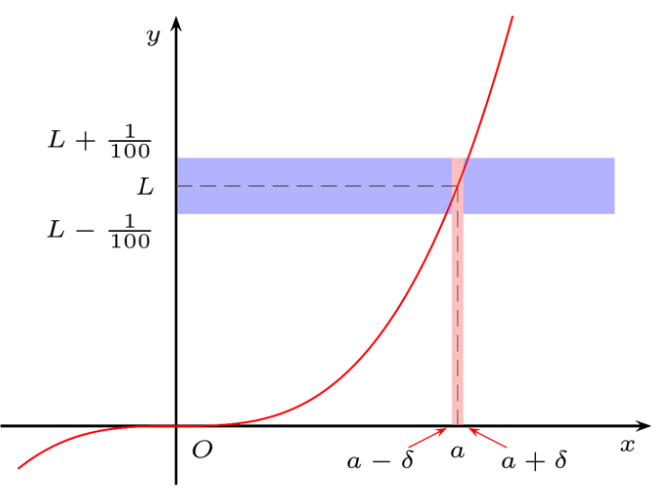
\includegraphics[width=0.9\linewidth]{ma1102r-limits.png}
\end{center}
informally,
\begin{itemize}
    \item $0 < \abs{x - a} < \delta \Then$ $x$ is close to but not equal to $a$.
    \item $0 < \abs{f(x) - L} < \epsilon \Then$ $f(x)$ is arbitrarily close to $L$.
\end{itemize}
% \begin{center}
%     if $f(x)$ is arbitrarily close to L by taking $x$ to be sufficiently close (but not equal to) $a$, then we write
%     \\* $\displaystyle{\lim_{x \to a} f(x) = L}$
%     \\* or $x \to a \Then f(x) \to L$
% \end{center}
% \begin{itemize}
%     \item the limit $\displaystyle{\lim_{x \to a} f(x)}$
%     \begin{itemize}
%         \item depends only on the values of $f(x)$ for $x$ near $a$    
%         \item is independent to the value of $f(x)$ at $a$.
%     \end{itemize}
% \end{itemize}

\subsection{limit laws}
\begin{itemize}
    \item Let $c \in \mathbb{R}$. $\displaystyle{\lim_{x \to a} c = c}$
    \item $\displaystyle{\lim_{x \to a} x = a}$
\end{itemize}
Suppose $\displaystyle{\lim_{x \to a} f(x) = L}$ and $\displaystyle{\lim_{x \to a} g(x) = M}$. Let $c$ be a constant. 
\begin{itemize}
    \item $\displaystyle{\lim_{x \to a} \left( cf(x) \right)} = cL = c \lim_{x \to a} f(x)$
    \item $\displaystyle{\lim_{x \to a} \left( f(x) + g(x) \right) = L + M = \lim_{x \to a} f(x) + \lim_{x \to a} g(x)}$
    \item $\displaystyle{\lim_{x \to a} \left( f(x) - g(x) \right) = \lim_{x \to a} f(x) - \lim_{x \to a} g(x)}$
    \item $\displaystyle{\lim_{x \to a} \left(f(x) g(x)\right) \lim_{x \to a} f(x) \lim_{x \to a} g(x)}$
    \item $\displaystyle{\lim_{x \to a} \frac{f(x)}{g(x)} = \frac{\lim_{x \to a} f(x)}{\lim_{x \to a} g(x)}}$ provided that $\displaystyle{\lim_{x \to a} g(x) \neq 0}$
    \item $\displaystyle{\lim_{x \to a} \left( f(x) \right) ^n = \left(\lim_{x \to a} f(x)\right)^n}$
    \item $\displaystyle{\lim_{x \to a} \sqrt[n]{f(x)} = \sqrt[n]{\lim_{x \to a} f(x)}}$
\end{itemize}

\begin{center}
    \fbox{
        if $\displaystyle{\lim_{x \to a} \frac{f(x)}{g(x)}}$ exists and $\displaystyle{\lim_{x \to a} g(x) = 0}$, then $\displaystyle{\lim_{x \to a} f(x) = 0}$
    }
\end{center}

\subsubsection{inequalities on limits}
Suppose $\displaystyle{\lim_{x \to a} f(x) = L}$ and $\displaystyle{\lim_{x \to a} g(x) = M}$. 
\begin{center}
    \textbf{lemma}
    \\* if $f(x) \leq g(x)$ for all $x$ near $a$ (except possibly at $a$), 
    \\* then $L \leq M$.

    \textbf{lemma}
    \\* If $f(x) \geq 0$ for all $x$, then $L \geq 0$.
\end{center}

\subsubsection{direct substitution property}
\begin{center}
    Let $f$ be a polynomial or rational function. 
    \\* If $a$ is in the domain of $f$, then
    \\* $\displaystyle{\lim_{x \to a} f(x) = f(a)}$

    If $f(x) = g(x)$ for all $x$ near $a$ except possibly at $a$, then 
    \\* $\displaystyle{\lim_{x \to a} f(x) = \lim_{x \to a} g(x)}$
\end{center}

applications
\begin{itemize}
    \item if $a$ is not in the domain (e.g. 0 denominator), don't apply directly
    \item convert to an equivalent function and then sub in
\end{itemize}

\subsection{one-sided limits}
\begin{itemize}
    \item limit laws also hold for one-sided limits
\end{itemize}
\begin{center}
    If as $x$ is close to $a$ from the right, $f(x)$ is close to L, the right-hand limit of $f$ as $x$ approaches $a$ equals $L$.
    \\* $\displaystyle{\left( x \to a^+ \Then f(x) \to L \right) \Then \lim_{x \to a^+} f(x) = L}$
    
    If as $x$ is close to $a$ from the left, $f(x)$ is close to L, the left-hand limit of $f$ as $x$ approaches $a$ equals $L$.
    \\* $\displaystyle{\left( x \to a^- \Then f(x) \to L \right) \Then \lim_{x \to a^-} f(x) = L}$
\end{center}

\begin{center}
    \fbox{
        $\displaystyle{\lim_{x \to a} f(x) = L \iff \lim_{x \to a^+} f(x) = \lim_{x \to a^-} f(x) = L}$
    }
    $f(x) \to L \Leftarrow x \to a \Iff \begin{cases}
        x \to a^+ \Then f(x) \to L \\
        x \to a^- \Then f(x) \to L
    \end{cases}$
\end{center}

\subsubsection{definition of one-sided limits}
\begin{center}
    \textbf{LH Limit}: $\displaystyle{\lim_{x \to a^-} f(x) = L}$ 
    \\* if for every $\epsilon > 0$ there exists $\delta > 0$ such that
    \\* $0 < a - x < \delta \Then \abs{f(x) - L} < \epsilon$
\end{center}
\begin{center}
    \textbf{RH Limit}: $\displaystyle{\lim_{x \to a^+} f(x) = L}$ 
    \\* if for every $\epsilon > 0$ there exists $\delta > 0$ such that
    \\* $0 < x - a < \delta \Then \abs{f(x) - L} < \epsilon$
\end{center}

\subsection{definition of infinite limits}
% \subsubsection{definition of infinite limit}
\begin{center}
    $\displaystyle{\lim_{x \to a} f(x) = \infty}$ 
    \\* if for every $M > 0$ there exists $\delta > 0$ such that
    \\* $0 < \abs{x - a} < \delta \Then f(x) > M$
    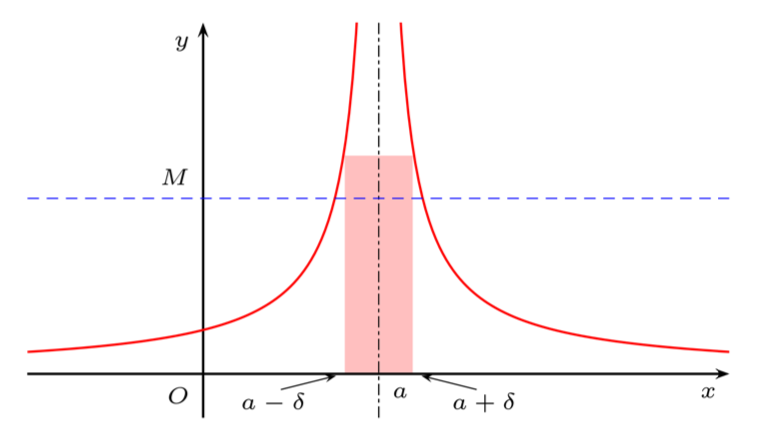
\includegraphics[width=0.9\linewidth]{ma1102r-infinite-limit.png}
    \\* \textbf{negative infinite limit:}
    \\* $0 < \abs{x - a} < \delta \Then f(x) < M$
\end{center}

\subsubsection{limits to infinity}
\begin{center}
    $\displaystyle{\lim_{x \to \infty}f(x) = L}$: 
    \\* For every $\epsilon > 0$, there exists $N$ such that
    \\* $x > N \Then \abs{f(x) - L} < \epsilon$
    \\ \ 
    \\ $\displaystyle{\lim_{x \to \infty}f(x) = \infty}$: 
    \\* For every $M > 0$, there exists $N$ such that
    \\* $x > N \Then f(x) > M$
\end{center}
% \begin{center}
%     Suppose $f$ is defined on both sides of $a$ (except possibly at $a$).
%     \\* If $f(x)$ is arbitrarily large by taking $x$ sufficiently close to $a$, 
%     \\* $\displaystyle{\lim_{x \to a} f(x) = \infty}$
%     \\* If $f(x)$ is arbitrarily negatively large $\cdots$, 
%     \\* $\displaystyle{\lim_{x \to a} f(x) = -\infty}$

%     Suppose $f$ is defined on $[M, \infty)$ for some real number $M$.
%     \\* If $f(x)$ is arbitrarily close to $L$ by taking $x$ sufficiently large,
%     \\* $\displaystyle{\lim_{x \to \infty} f(x) = L}$
% \end{center}

\subsection{squeeze theorem}
\begin{itemize}
    \item Suppose $f(x)$ is bounded by $g(x)$ and $h(x)$ where 
    \begin{itemize}
        \item $g(x) \leq f(x) \leq h(x)$ for all $x$ near $a$ (except at $a$),
        \item and $\displaystyle{\lim_{x \to a} g(x) = \lim_{x \to a} h(x) = L}$.
    \end{itemize}
\end{itemize}
\centerline{Then $\displaystyle{\lim_{x \to a} f(x) = L}$}


\section{02. CONTINUOUS FUNCTIONS}
\subsection{definition of continuity}
\begin{center}
    a function $f$ is \textbf{continuous at $a$} $\Iff$ 
    \\* $f$ is continuous from the left and from the right at $a$.
    \\* $\displaystyle{\lim_{x \to a} f(x) = f(a)}$
\end{center}
a function $f$ is \textit{continuous at an interval} if it is continuous at every number in the interval.
\begin{center}
    $f$ is continuous on \textbf{open interval} $(a, b)$
    \\* $\Iff f$ is continuous at every $x \in (a, b)$
    \\ $f$ is continuous on \textbf{closed interval} [a, b]
    $\Iff \begin{cases}
        f $ is continuous at every $x \in (a, b) \\
        f $ is continuous from the right at $ a \\
        f $ is continuous from the left at $ b
    \end{cases}$
\end{center}

\subsubsection{continuity test}
$f$ is continuous at $a \Iff$ 
\begin{enumerate}
    \item $f$ is defined at $a$ ($a$ is in the domain of $f$)
    \item $\displaystyle{\lim_{x \to a} f(x)}$ exists
    \item $\displaystyle{\lim_{x \to a} f(x)} = f(a)$ 
\end{enumerate}

\subsubsection{precise definition of continuity}
\begin{center}
    a function $f$ is continuous at a number $a$ if $\forall \epsilon > 0, \exists \delta > 0$ such that 
    $\abs{x - a} < \delta \Then \abs{f(x) - f(a)} < \epsilon$
\end{center}

\subsubsection{examples of discontinuity}
\begin{itemize}
    \item removable discontinuity
    \item infinite discontinuity
    \item jump discontinuity
\end{itemize}

\subsection{properties of continuous functions}
let $f$ and $g$ be functions continuous at $a$. let $c$ be a constant.
\begin{enumerate}
    \item $cf$ is continuous at $a$
    \item $f+g$ is continuous at $a$
    \item $f-g$ is continuous at $a$
    \item $fg$ is continuous at $a$
    \item $\frac{f}{g}$ is continuous at $a$, provided $g(a) \neq 0$
\end{enumerate}

\textbf{other properties}
\begin{itemize}
    \item a polynomial is continuous everywhere;
    \item a rational function is continuous on its domain
    \item let $c$ be a real number. $f(x) = c$ is continuous on $\mathbb{R}$.
    \item $f(x) = x$ is continuous on $\mathbb{R}$.
\end{itemize}

\subsubsection{trigonometric functions}
\begin{itemize}
    \item $f(x) = \sin x$  and $g(x) = \cos x$ are continuous everywhere
    \item $\tan x, \sec x$ are continuous whenever $\cos x \neq 0$
    \item $\cot x, \csc x$ are continuous whenever $\sin x \neq 0$
    \begin{itemize}
        \item domain: $\mathbb{R} \backslash \{0, \pm \pi, \pm 2\pi, \cdots\}$
    \end{itemize}
\end{itemize}

\subsection{composite of continuous functions}
\begin{center}
    if $f$ is continuous at $b$ and $\displaystyle{\lim_{x \to a} g(x) = b}$, then 
    \\* $\displaystyle{\lim_{x \to a} f(g(x)) = f(\lim_{x \to a} g(x))}$
\end{center}
\begin{center}
    if $g$ is continuous at $a$ and $f$ is continuous at $g(a)$,
    \\* then $f \circ g$ is continuous at $a$.
    \\* $\displaystyle{\lim_{x \to a} (f \circ g)(x) = (f \circ g)(a)}$
\end{center}

\subsection{substitution theorem}
Suppose $y = f(x)$ such that $\displaystyle{\lim_{x \to a}f(x) = b}$. If
\begin{enumerate}
    \item $g$ is continuous at $b$, OR 
    \item $\forall x$ near $a$, except at $a$, $f(x) \neq b$ and $\displaystyle{\lim_{y \to b} g(y)}$ exists
\end{enumerate}
Then $\displaystyle{\lim_{x \to a} g(f(x)) = \lim_{y \to b} g(y)}$

\subsection{intermediate value theorem}\
\begin{center}
    Let $f$ be a function continuous on $[a, b]$ with $f(a) \neq f(b)$. 
    \\* Let $N$ be a number between $f(a)$ and $f(b)$.
    \\* Then there exists $c \in (a, b)$ such that $f(c) = N$.
    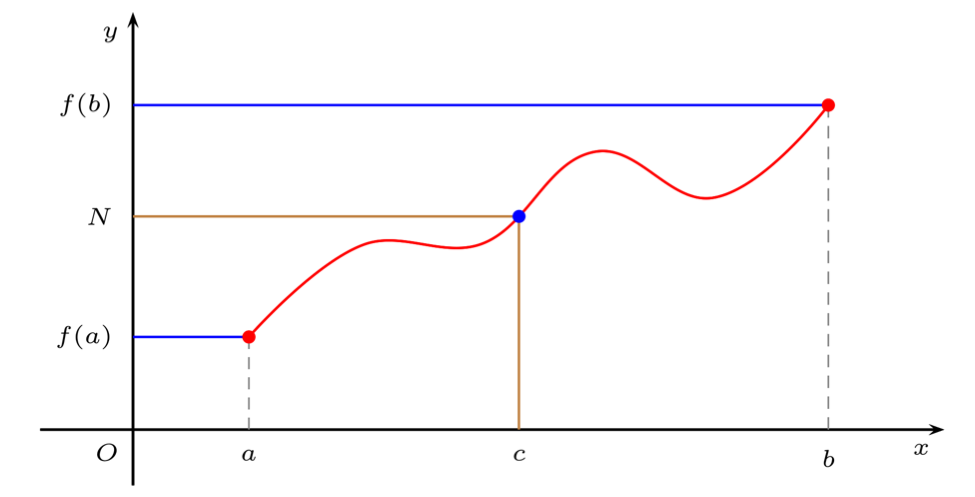
\includegraphics[width=0.9\linewidth]{ma1102r-intermediate-value-theorem.png}
\end{center}

\section{03. DERIVATIVES}

\subsection{tangent line}
\begin{center}
    the \textbf{tangent line} to $y=f(x)$ at $(a, f(a))$ is the line 
    \\* passing through $(a, f(a))$ with slope $f'(a)$:
    \\* $y = f'(a)(x-a) + f(a)$
\end{center}

\subsection{definition of derivatives}
\begin{itemize}
    \item $f$ is differentiable at $a$ if $f'(a)$ exists
    \item $f'(a)$ is the slope of $y=f(x)$ at $x=a$
\end{itemize}
\begin{center}
    $\displaystyle{f'(x) := \lim_{h \to 0} \frac{f(x+h) - f(x)}{h}}$
    $\displaystyle{f'(a) := \lim_{x \to a} \frac{f(x) - f(a)}{x-a}}$
\end{center}
\begin{itemize}
    \item $f'(x) = y' = \frac{dy}{dx} = \frac{df}{dx} = \frac{d}{dx}f(x) = D_xf(x) = \cdots$
    \item $\displaystyle{\frac{dy}{dx} := \lim_{x \to 0} \frac{\Delta y}{\Delta x}}$  (derivative of $y$ with respect to $x$)
    \item $f'(a) = \frac{dy}{dx}\vert_{x = a}$
\end{itemize}

\subsection{differentiable functions}
\begin{itemize}
    \item $f$ is differentiable at $a$ if $\displaystyle{f'(a) := \lim_{x \to 0}\frac{f(a + h) - f(a)}{h}}$ exists.
    \item $f$ is differentiable on $(a, b)$ if $f$ is differentiable at every $c \in (a, b)$
\end{itemize}

\subsubsection{differentiability \& continuity}
\begin{itemize}
    \item if $f$ is differentiable at $a$, then $f$ is continuous at $a$.
    \begin{itemize}
        \item differentiability $\Then$ continuity
    \end{itemize}
    \item continuity $\nRightarrow$ differentiability
\end{itemize}

\subsection{differentiation}
\begin{itemize}
    \item every polynomial and rational function is differentiable on its domain
    \begin{itemize}
        \item the domain of $f'$ may be smaller than the domain of $f$.
    \end{itemize}
    \item trigonometric functions are differentiable on the domain
\end{itemize}

\subsubsection{chain rule}
\begin{center}
    If $g$ is differentiable at $a$ and $f$ is differentiable at $b = g(a)$, then $F = f \circ g$ is differentiable at $a$ and
    \\* $F'(a) = (f \circ g)'(a) = f'(b)g'(a) = f'(g(a))g'(a)$
\end{center}
\begin{center}
    If $z=f(y)$ and $y = g(x)$, then 
    \\* $\frac{dz}{dx} = \frac{dz}{dy} \frac{dy}{dx}$
    \\* $\frac{dz}{dx}\vert_{x=a} = \frac{dz}{dy}\vert_{y=b} \frac{dy}{dx}\vert_{x=a}$
\end{center}

\subsubsection{generalised chain rule}
$h$ is differentiable at $a$; $g$ is differentiable at $B = h(a)$; $f$ is differentiable at $c = g(b)$.
\begin{align*}
    (f \circ (g \circ h))'&= f' \circ (g \circ h) \cdot (g \circ h)'
    \\ &= f'(c)g'(b)h'(a)
\end{align*}
\begin{center}
    Leibniz notation:
    \\* If $y = h(x), z=g(y), w=f(z)$,
    \\* $\frac{dw}{dx}  = \frac{dw}{dz} \frac{dz}{dy} \frac{dy}{dx}$
\end{center}

\subsection{implicit differentiation}
\begin{itemize}
    \item assumes that $\frac{dy}{dx}$ exists
\end{itemize}

\subsection{second derivative}
\begin{center}
    $f''(x) = \frac{d}{dx}(\frac{dy}{dx}) = \frac{d^2y}{dx^2}$
    \\* $f' = D(f) \Rightarrow f'' := D^2(f)$
\end{center}

\subsection{higher derivatives}
\begin{center}
    $f^{(0)} := f$
    \\* For any positive integer $n$, $f^{(n)} := (f^{(n-1)})'$
    \\* if $y=f(x)$, then $f^{(n)}(x) = y^{(n)} = \frac{d^ny}{dx^n} = D^nf(x)$
\end{center}


\begin{center}
    \ 
\end{center}







\subsection{misc}
\subsubsection{triangle inequality}
\begin{center}
    $\abs{a = b} \leq \abs{a} + \abs{b}$ for all $a, b \in \mathbb{R}$
\end{center}

\subsubsection{binomial theorem}
\begin{center}
    $\displaystyle{(a+b)^n = \sum^n_{k=0}\binom{n}{k}a^{n-k}b^k}$
    \\* $= a^n + \binom{n}{1}a^{n-1}{b} + \dots + \binom{n}{n-1} ab^{n-1} + b^n$
\end{center}
\begin{center}
    where the binomial coefficient is given by 
    \\* $\binom{n}{k} = \frac{n!}{k!(n-k)!}$
\end{center}

\subsubsection{factorisation}
\begin{center}
    $a^n-b^n = (a-b)(a^{n-1} + a^{n-2}b + \cdots + ab^{n-2} + b^{n-1})$
\end{center}

\end{multicols*}

\end{document}